\begin{definition}[language (or type) of algebras] A language or type of
algebras is a set $\mathcal{F}$ of function symbols, such that a nonnegative
integer $n$ is assigned to each member $f$ of $\mathcal{F}$. This integer is
called the arity of $f$, and $f$ is said to be an n-ary function symbol.
\end{definition}

\begin{remark} There can be several functions $f$ with the same arity (in fact,
they are in the same subset $\mathcal{F}_n$)
\end{remark}


\begin{definition}[algebra] Let $A$ be a nonempty set, let $F$ be family of
finitary operations on $A$ indexed by the language $\mathcal{F}$: that is, for
every operation $f \in \mathcal{F}$ there is an operation $f^{A} \in F$.

  An operation can be either a function, when the arity of $f$ is greater than
$0$, or a constant, when it is equal to $0$.

  An algebra \textbf{A} is a ordered pair $<A,F>$: here, $A$ is called the
universe (or underlying set) of $\boldsymbol{A}= <A,F>$ and the
$f^{\boldsymbol{A}}$'s are called the fundamental operations of
$\boldsymbol{A}$.
\end{definition}

\begin{remark} if $\mathcal{F}$ is finite, we often write an algebra
$\boldsymbol{A} = <A, f_1,...,f_k>$. Take for instance any ring $<A,+,
\times>$.
\end{remark}

\begin{remark} Many of the algebras we are used to working with do not have
fundamental operations of arity greater than two.
\end{remark}

\begin{example} We are going to give examples of different kind of algebras
  \begin{definition}[group] A group $G$ is an algebra $<G, \cdot, ^{-1},1>$ with
a binary, a unary, and a nullary operation - in which the following identities
are true:
    \begin{enumerate}
    \item $x \cdot (y \cdot z) \approx (x \cdot y) \cdot z$ (Associativity)
    \item $x \cdot 1 \approx 1 \cdot x \approx x$ (Identity element)
    \item $x \cdot x^{-1} \approx x^{-1} \cdot x \approx 1$ (Inverse element)
    \end{enumerate}

    A group $G$ is Abelian (or commutative) if $x \cdot y \approx y \cdot x$.
  \end{definition}

  \begin{definition}[subgroup]
    Let $\boldsymbol{G}$ be a group under binary operation $\cdot$. A subset $H$
    of $G$ is called a subgroup of $\boldsymbol{G}$ if $\boldsymbol{H}$ also
    forms a group under the operation $\cdot$.
  \end{definition}

  \begin{definition}[normal subgroup]
    Let $G$ be a group. We say $H$ is a \textbf{normal subgroup} of $G$ if
    \begin{equation}
      \label{eq:subgroup}
      \forall h \in H, \forall x \in G, xhx^{-1} \in H
    \end{equation}
  \end{definition}

  \begin{example}
    Let $G$ be a group. $\{1\}$ is a normal subgroup of $G$ given that $\forall x \in G$, $x1x^{-1} = xx^{-1} = 1 \in G$.
  \end{example}

  \begin{remark} The notation $1$ for the nullary operation is not very clear:
for example, for the Abelian group $<\mathbb{Z}, +>$, the sum of an element with
its inverse is not $1$ but $0$ (Inverse element law).
  \end{remark}

  \begin{definition}[groupoid] A groupoid is an algebraic structure consisting
of an nonempty set $G$ and the binary partial function $\cdot$ defined on a
subset of $G$ (not necessarily defined for all pair of elements in $G$).
  \end{definition}

  \begin{definition}[semigroup] A semigroup is a groupoid $<G,\cdot>$ which
verifies associativity. It is commutative (or Abelian) if it verifies
commutativity.
  \end{definition}

  \begin{definition}[ring] A ring is an algebra $<R,+, \cdot, -, 0>$ where $+$
and $\cdot$ are binary, $-$ is unary and $0$ is nullary.
    \begin{enumerate}
    \item $<R,+, \cdot, -, 0>$ is an Abelian group.
    \item $<R,\cdot>$ is a semigroup
    \item It verifies distributivity
    \end{enumerate}
  \end{definition}

  \begin{remark} We can also build a ring with identity with an nullary
(constant) operation $1$ verifying the properties of a ring plus the second
property of a group.
  \end{remark}

  \begin{definition}[semillatice] A semillattice is a semigroup $<S,\cdot>$
which satisfies the commutative law and the idempotent law: $x \cdot x \approx
x$.
  \end{definition}

\end{example}

\begin{property}[similar algebras]
  Algebras $\boldsymbol{A}$ and $\boldsymbol{B}$ are said to be similar if and
  only if they are of the same type $\mathcal{F}$. We say that they belong to
  the same class of algebras $K$.

  \begin{question}
    Are they really?
  \end{question}

\end{property}




\subsection{Isomorphic Algebras}

\begin{definition}[isomorphism] Let $\boldsymbol{A}$ and $\boldsymbol{B}$ be two
algebras of the same language $\mathcal{F}$. Then a function $\alpha: A
\rightarrow B$ is an isomorphism from $\boldsymbol{A}$ to $\boldsymbol{B}$ if
$\alpha$ is bijective and, for any n-ary function $f \in \mathcal{F}$, for
$a_1,...,a_n \in A$, we have:
  \begin{equation}
    \label{eq:morphism} \alpha (f^{\boldsymbol{A}}(a_1,...,a_n)) =
f^{\boldsymbol{B}}(\alpha(a_1),...,\alpha(a_n))
  \end{equation}

  We say $\boldsymbol{A}$ is isomorphic to $\boldsymbol{B}$, written
$\boldsymbol{A} \cong \boldsymbol{B}$ if there is an isomorphism from
$\boldsymbol{A}$ to $\boldsymbol{B}$.
\end{definition}

\subsection{Subuniverse / Subalgebras}

\begin{definition}[closed] Let $A$ be a nonempty set, and an operation $f: A^n
\rightarrow A$ of arity $n$. We say that $A$ is \textbf{closed} with respect to
$f$ (or $f$ \textbf{preserves $A$}) if and only if $\forall a_1,...,a_n \in A$,
$f(a_1,...,a_n) \in A$.
\end{definition}

\begin{remark} If $f$ is a constant, this means that $A$ is closed to respect to
$f$ if and only if $f \in A$.
\end{remark}

\begin{example} Let's consider the following sets, along with the addition
function $+$:$[0,100], \mathbb{N}$. $\mathbb{N}$ is closed in respect to $+$:
any pair of numbers in $\mathbb{N}$ we choose to add will stay in
$\mathbb{N}$. But for $[0,100]$, $50 + 60 = 110$ and $110 \notin [0,100]$: so
$[0,100]$ isn't closed in respect to $+$.
\end{example}

\begin{definition}[subuniverse] Let $\boldsymbol{A}$ be an algebra. We say a
subset of $A$ is a \textbf{subuniverse} if it is closed with respect of every
basic operation of $\boldsymbol{A}$.
\end{definition}

\begin{example} Let $\boldsymbol{\mathbb{Z}}$, $\boldsymbol{\mathbb{N}}$, and
$\boldsymbol{\mathbb{N}_{[0,100]}}$ be algebras defined over the $+$ (addition)
operation. We have $\boldsymbol{\mathbb{N}_{[0,100]}} \subseteq
\boldsymbol{\mathbb{N}} \subseteq \boldsymbol{\mathbb{Z}}$.  $\mathbb{N}$ is
closed in respect to $+$: any pair of numbers in $\mathbb{N}$ we choose to add
will stay in $\mathbb{N}$: as such, it is subuniverse of
$\boldsymbol{\mathbb{Z}}$. But for $[0,100]$, $50 + 60 = 110$ and $110 \notin
[0,100]$: so $[0,100]$ isn't closed in respect to $+$ - and it isn't a
subuniverse of $\boldsymbol{\mathbb{Z}}$.
\end{example}

\begin{definition}[subalgebra] Let $\boldsymbol{A},\boldsymbol{B}$ be two
algebras of the same type. $\boldsymbol{B}$ is a subalgebra of $\boldsymbol{A}$
if $B$ is a nonempty subuniverse of $\boldsymbol{A}$ and, for every operation
symbol $f_t$ of rank $n$ in type $\tau$ of $\boldsymbol{A}$:
  \begin{equation}
    \label{eq:subalgebra} f^{B}(a_1,...,a_n) = f^{A}(a_1,...,a_n) \text{ for all
} a_1,...,a_n \in B
  \end{equation}

  Then, $f^{B}$ is called the restriction of $f^{A}$ to $B$.
\end{definition}

\begin{remark} The conditions on the operations of a subalgebra are the same as
those required to build a subuniverse that is closed.
\end{remark}

\begin{definition}[embedding]  Let $\boldsymbol{A}$ and $\boldsymbol{B}$ be
two algebras of the same type. Then a function $\alpha: A \rightarrow B$ is an
embedding from $\boldsymbol{A}$ to $\boldsymbol{B}$ if $\alpha$ is injective and
it verifies equation \ref{eq:morphism}.
\end{definition}

\begin{remark}  For brevity, we cay $\alpha: \boldsymbol{A} \rightarrow
\boldsymbol{B}$ is an embedding.
\end{remark}

\begin{theorem}  If $\alpha: \boldsymbol{A} \rightarrow \boldsymbol{B}$ is an
embedding, then $\alpha(A)$ is a subuniverse of $\boldsymbol{B}$.
\end{theorem}

\begin{proof}
  $\forall a_1,...,a_n \in A$, we have $f^{\boldsymbol{A}}(a_1,...,a_n) \in A$
  (since $\boldsymbol{A}$ is an algebra, so its operations $f^{\boldsymbol{A}}$ are closed in $A$), so
  $\alpha(f^{\boldsymbol{A}}(a_1,...,a_n)) \in \alpha(A)$.

  Since $\alpha$ is an embedding, we have the following equality, $\forall a_1,...,a_n \in A$:
    \begin{equation}
      \alpha (f^{\boldsymbol{A}}(a_1,...,a_n)) =
      f^{\boldsymbol{B}}(\alpha(a_1),...,\alpha(a_n))
  \end{equation}

  $\alpha (f^{\boldsymbol{A}}(a_1,...,a_n)) \in \alpha(A)$, as seen
  previously. By the previous equation, since both expressions are equal,
  $f^{\boldsymbol{B}}(\alpha(a_1),...,\alpha(a_n)) \in \alpha(A)$: this shows
  that operations $f^{\boldsymbol{B}}$ of $B$ are closed for elements of
  $\alpha(A)$.

  By the definition of a subuniverse, since $\alpha(A)$ is closed in regards to
  operations of $B$, $\alpha(A)$ is a subuniverse of $\boldsymbol{B}$.


\end{proof}

\begin{definition}  If $\alpha: \boldsymbol{A} \rightarrow \boldsymbol{B}$ is
an embedding, $\alpha(\boldsymbol{A})$ denotes the subalgebra of
$\boldsymbol{B}$ with universe $\alpha(A)$.
\end{definition}

\begin{notation} We denote by $Sub(A)$ the set of all subuniverses of
$\boldsymbol{A}$.
\end{notation}

\subsection{Algebraic Lattices and Subuniverses}

\begin{definition}[closure] If we are given a set $A$, a mapping $C:
\mathbb{P}(A) \rightarrow \mathbb{P}(A)$ (where $\mathbb{P}(A)$ is the power set
of $A$) is called a closure operator on $A$, if for $X,Y \subseteq A$, it
satisfies:
  \begin{enumerate}
  \item $X \subseteq C(X)$ (extensive)
  \item $C(C(X)) = C(X)$ (idempotent)
  \item $X \subseteq Y$ implies $C(X) \subseteq C(Y)$ (isotone)
  \end{enumerate}

  A subset $X$ of $A$ is called a \textbf{closed subset} if $C(X) = X$. The
poset of closed subsets of $A$, with set inclusion as the partial ordering, is
denoted by $L_C$.
\end{definition}

\begin{definition}[algebraic closure] A closure operator $C$ on the set $A$ is
an \textbf{algebraic closure operator} if for every $X \subseteq A$:

	\begin{equation}
		\label{eq:closure} C(X) = \bigcup \{ C(Y) : Y \subseteq X \text{ and $Y$
is finite} \}
	\end{equation}
\end{definition}

\begin{remark} Extensive, Idempotent and proprety \ref{eq:closure} entails the
isotone law.
\end{remark}


\begin{definition}[generated subuniverse] Given an algebra $\boldsymbol{A}$
define, for every $X \subseteq A$,

	\begin{equation} Sg(X) = \bigcap \{ B : X \subseteq B \text{ and $B$ is a
subuniverse of $\boldsymbol{A}$}\}
	\end{equation}

	We read $Sg(X)$ as "the subuniverse generated by X".
\end{definition}

\begin{remark} This definition states that the generated subuniverse of a subset
$X$ of $A$ is the smallest subuniverse in $A$ that contains $X$. As such, it is
analogue to a topological closure (adherence in french)
\end{remark}

\begin{theorem} If we are given an algebra $\boldsymbol{A}$ then Sg is an
algebraic closure operator on $A$.
\end{theorem}

\begin{proof}
	TODO
\end{proof}

\begin{corollary}
  If $\boldsymbol{A}$ is an algebra, then $\boldsymbol{L_{Sg}}$, the lattice of subuniverses of $\boldsymbol{A}$, is an algebraic lattice.
\end{corollary}

\begin{notation}
	Given an algebra $\boldsymbol{A}$, $Sub(\boldsymbol{A})$ denotes the \textbf{set of subuniverses} of $\boldsymbol{A}$. $\boldsymbol{Sub}(\boldsymbol{A})$ is the \textbf{corresponding algebraic lattice}, the \textbf{lattice of subuniverses} of $\boldsymbol{A}$.
\end{notation}

\begin{definition}[generated algebra]
	For $X \subseteq A$, we say \textbf{$X$ generated $\boldsymbol{A}$} (or $\boldsymbol{A}$ is \textbf{generated by} $X$, or $X$ is a \textbf{set of generators} of $\boldsymbol{A}$) if $Sg(X) = A$.

	The algebra $\boldsymbol{A}$ is \textbf{finitely generated} if it has a finite set of generators.
\end{definition}

\begin{theorem}[Birkhoff and Frink]
  If $\boldsymbol{L}$ is an algebraic lattice, then
  $L \cong \boldsymbol{Sub}(\boldsymbol{A})$ for some algebra $\boldsymbol{A}$.
\end{theorem}

\begin{proof}

\end{proof}

\subsection{Equivalence classes}

\begin{definition}[equivalence class] Given a set $S$ and an equivalence
relation $\theta$ on $S$, the equivalence class of an element $a \in S$, denoted
by $[a]$, is the set $\{x \in S | x \theta a\}$.
\end{definition}

\begin{notation}
  We can choose to specify the equivalence relation for a given equivalence
  class: here, $[a] = [a]_{\theta}$.
\end{notation}

\begin{prop} If $\theta$ is an equivalence relation on a set $S$ then $a \theta
b \implies [a] = [b]$.
\end{prop}

\begin{proof} Let's show that $a \theta b \implies [a] = [b]$ if $\theta$ is an
equivalence relation.

  Let's suppose $a \theta b$. We will show $[a] \subseteq [b]$ and $[b]
\subseteq [a]$.

  Let $x \in [a]$, so $x \theta a$. We have $x \theta a$ and $a \theta b$, so by
transitivity of the equivalence relation, $x \theta b \implies x \in [b]$. We
have shown $x \in [a] \implies x \in [b]$, so $[a] \subseteq [b]$.

  Let $x \in [b]$, so $x \theta b$. We have $a \theta b \implies b \theta a$, by
symmetry of the equivalence relation, so $x \theta b$ and $b \theta a$ implies
$x \theta a$ proving $x \in [a]$. Thus $[b] \subseteq [a]$.
\end{proof}

\begin{lemma} Given an equivalence relation $\theta$ on a set $S$, if $a,b \in
S$ then either $[a] \cap [b] = \emptyset$ or $[a] = [b]$.
\end{lemma}

\begin{theorem} If $\theta$ is an equivalence relation on any nonempty set $A$,
then the distinct set of equivalence classes of $\theta$ forms a partition of
$A$.
\end{theorem}

\begin{proof} Let $A_1, ...,A_n$ denote the equivalence classes of a nonempty
set $A$. We must prove that $\bigcup A_i = A$ and that $\bigcap A_i = \emptyset$
in order for $A_1, ...,A_n$ to be a partition of $A$.

Let's show that $\bigcup A_i = A$: we will show $\bigcup A_i \subseteq A$ and $A
\subseteq \bigcup A_i$.

Let $x \in \bigcup A_i$, so $\exists i$ such that $x \in A_i$, by definition of
the union. Since $A_i = \{x \in A | x \theta a_i\}$, where $[a_i] = A_i$, we
have $x \in A_i \implies x \in A$.

Now let $x \in A$. We have $x \in [x]$, by reflexivity of the equivalence
relation, and by definition of the set of equivalence classes $\exists i$ such
that $[x] = A_i$. Therefore, $x \in \bigcup A_i$ since $[x] = A_i \iff x \in
A_i$.

Now let's show that $\bigcap A_i = \emptyset$.

By definition of the set of equivalence classes, $A_i \neq A_j$, for $i \neq j$
given that they are disjoint. Therefore, by the previous lemma, $A_i \cap A_j =
\emptyset$, for $i \neq j$. This proves that $\bigcap A_i = \emptyset$.
\end{proof}

\begin{notation} The partition formed by the equivalence classes is the quotient
set, and is denoted by $S / \theta$.
\end{notation}

\subsection{Congruences and Quotient Algebras}

\begin{definition}[congruence] Let $\boldsymbol{A}$ be an algebra of type
$\mathcal{F}$, and let $\theta \in Eq(A)$. Then $\theta$ is a
\textbf{congruence} on $\boldsymbol{A}$ if $\theta$ satisfies the following
property:

  \begin{property}[compatibilty property]
    \label{prop:compatibility} For each $n$-ary function symbol $f \in
\mathcal{F}$ and elements $a_i, b_i \in A$, if $a_i \theta b_i$ holds for $1
\leq i \leq n$ then:
    $$f^{\boldsymbol{A}}(a_1,...,a_n) \theta f^{\boldsymbol{A}}(b_1,...,b_n)$$
    holds.
  \end{property}

\end{definition}

\begin{notation} We denote by $Con \boldsymbol{A}$ the set of all congruences on
an algebra $\boldsymbol{A}$.
\end{notation}

\begin{definition}[quotient algebra] Let $\theta$ be a congruence on an algebra
$\boldsymbol{A}$. Then the \textbf{quotient algebra} of $\boldsymbol{A}$ by
$\theta$, written $\boldsymbol{A} / \theta$, is the algebra whose universe is $A
/ \theta$ and whose fundamental operations satisfy:
  \begin{equation} f^{\boldsymbol{A} / \theta} (a_1 / \theta, ..., a_n / \theta)
= f^{\boldsymbol{A}} (a_1, ..., a_n) / \theta
  \end{equation}

  where $a_1,...,a_n \in A$ and $f$ is an $n$-ary function symbol in
$\mathcal{F}$.
\end{definition}

\begin{remark}
  $a_1 / \theta$ is the equivalence class of $a_1$ in $A$ with the $\theta$ equivalence relation. We have
  $a_1 / \theta = [a_1]_{\theta} = \{a \in A | a \theta a_1\}$.
\end{remark}

\begin{remark} Intuitively, a quotient algebra is the result of partitionning
the elements of the algebra using a congruence relation. Here, the congruence
relation must be an equivalence relation that is additionnaly compatible with
all the operations of the algebra. (property \ref{prop:compatibility})
\end{remark}

\begin{example}
  Let $\boldsymbol{G}$ be a group. Then one can establish the following
  connection between congruences on $\boldsymbol{G}$ and normal subgroups of
  $\boldsymbol{G}$:
  \begin{enumerate}
  \item If $\theta \in Con \boldsymbol{G}$ then $1 / \theta$ is the universe of
    a normal subgroup of $\boldsymbol{G}$ and for $a,b \in G$, we have
    $a \theta b$ if and only if $ab^{-1} \in 1 / \theta$.

    \begin{proof}
      Let $\boldsymbol{G} = <G, \cdot, ^{-1},1>$ be a group, $\theta \in Con \boldsymbol{G}$ and $a,b \in G$.

      Let's prove that $1 / \theta$ is the universe of a normal subgroup of $\boldsymbol{G}$. Let $a_1, b_1, a_2, b_2, a_3, b_3 \in G$.

      By the compatibility property, we have:
      \begin{equation}
        \begin{dcases}
        a_1 \theta b_1 \\
        a_2 \theta b_2 \\
        a_3 \theta b_3 \end{dcases}
      \; \xRightarrow{} \;
      a_1 \cdot a_2 \cdot a_3 \: \theta \: b_1 \cdot b_2 \cdot b_3
    \end{equation}

    Let $h \in 1 / \theta = [1]_{\theta}$, and $x \in G$. We then choose $a_1 = x$, $a_2 = h$, $a_3 = x^{-1}$ and $b_1 = x$, $b_2 = 1$, $b_3 = x^{-1}$

    By reflexivity of the equivalence relation, $a_1 \theta b_1$ and
    $a_3 \theta b_3$. Given that $h \in 1 / \theta$, we also have
    $a_2 \theta b_2$. Therefore, $x \cdot h \cdot x^{-1} \theta x \cdot 1 \cdot x^{-1}$

    We have $x \cdot 1 = x$ and $x \cdot x^{-1} = 1$, by the properties of the
    identity and inverse elements in groups, so
    $x \cdot h \cdot x^{-1} \theta 1$ which proves
    $x \cdot h \cdot x^{-1} \in 1 / \theta$. By definition of a normal subgroup,
    $1 / \theta$ is a normal subgroup of $G$.

    Let's now prove that $a \theta b \iff a \cdot b^{-1} \in 1 / \theta$.

    Let $a \theta b$. By reflexivity of the equivalence relation we have
    $b^{-1} \theta b^{-1}$.

    By the compatibility property we have
    $a \cdot b^{-1} \: \theta \: b \cdot b^{-1}$. By the property of the
    inverse element in groups, $b \cdot b^{-1} = 1$. So $a \cdot b^{-1} \in 1 / \theta$. We have
    proven $a \theta b \implies a \cdot b^{-1} \in 1 / \theta$.

    Let $a \cdot b^{-1} \in 1 / \theta$ so $a \cdot b^{-1} \: \theta \: 1$. By
    the compatibility property, $a \cdot b^{-1} \cdot b \: \theta \: 1 \cdot
    b$. Therefore, by the properties of the equivalence relation, $a \theta b$.

    As such, we have proven $a \theta b \iff a \cdot b^{-1} \in 1 / \theta$.
  \end{proof}

\item If $\boldsymbol{N}$ is normal subgroup of $\boldsymbol{G}$ then the
  binary relation defined on $G$ by $a \theta b$ if and only if
  $a \cdot b^{-1} \in N$ is a congruence on $\boldsymbol{G}$ with $1 / \theta = N$.

  \begin{proof}
    To show that $\theta$ is a congruence on $G$, we will first show that it is
    an equivalence relation and then that it verifies the compatibility property.

    To show that $\theta$ is an equivalence relation, we will show that it is
    reflexive, symmetric and transitive.

    Let $N$ be a subgroup of $G$, and $\theta$ a binary relation defined on $G$
    by $a \theta b \iff a \cdot b^{-1} \in N$.

    \begin{enumerate}
    \item reflexivity ($a \theta a$): since $N$ is a subgroup, it posesses the
      identity element $1$ (since it verifies the properties of a group). By the
      properties of the inverse element in a group, we have
      $a \cdot a^{-1} = 1$. Therefore, $a \cdot a^{-1} \in N$.
    \item symmetry ($a \theta b \implies b \theta a$): suppose $a \theta b$,
      then $a \cdot b^{-1} \in N$. Therefore, $\exists h \in N$ such that
      $a \cdot b^{-1} = h$. We have:
      $$a = h \cdot b \iff 1 = h \cdot b \cdot a^{-1} \iff h^{-1} = b \cdot a^{-1}$$

      As such, given that $h^{-1} \in N$ since $N$ is a group, $b \theta a$.
    \item transitivity ($a \theta b$ and $b \theta c$ implies $a \theta c$):

      \begin{equation}
        \begin{dcases}
          a \cdot b^{-1} \in N   \\
          b \cdot c^{-1} \in N \end{dcases}
        \; \xRightarrow{} \;
        \begin{dcases}
          \exists h \in N, a \cdot b^{-1} = h \\
          \exists h^{'} \in N, b \cdot c^{-1} = h^{'}\end{dcases}
      \end{equation}

      Therefore, $a \cdot b^{-1} \cdot b \cdot c^{-1} = h \cdot h^{'}$ and
      $a \cdot b^{-1} \cdot b \cdot c^{-1} = a \cdot c^{-1}$. Given that
      $h \cdot h^{'} \in N$, we have $a \theta c$.
    \end{enumerate}

    Let's now prove the compatibility property for $\theta$. We will introduce a preliminary lemma
    \begin{lemma}
      Let $\boldsymbol{N}$ a normal subgroup of $\boldsymbol{G}$. We have:
      \begin{equation}
        \forall x \in G, \forall h \in N, \exists h^{'} \in N: x \cdot h = h^{'} \cdot x
      \end{equation}
    \end{lemma}

    \begin{proof}
      $\forall x \in G$, $\forall h \in N$, $\exists h^{'} \in N$ such that
      $x \cdot h \cdot x^{-1} = h^{'}$.  We have
      $( x \cdot h \cdot x^{-1} ) \cdot x = h^{'} \cdot x$, so $x \cdot h = h^{'} \cdot x$.
    \end{proof}

    Let's continue. Let $a_1, b_1, a_2, b_2 \in G$. We want to prove that
    $a_1 \theta b_1$ and $a_2 \theta b_2$ implies $a_1 \cdot a_2 \theta b_1 \cdot b_2$.

    \begin{equation}
      \begin{dcases}
        a_1 \cdot b_1^{-1} \in N   \\
        a_2 \cdot b_2^{-1} \in N \end{dcases}
      \; \xRightarrow{} \;
      \begin{dcases}
        \exists h_1 \in N, a_1 \cdot b_1^{-1} = h_1 \text{ (1)} \\
        \exists h_2 \in N, a_2 \cdot b_2^{-1} = h_2 \text{ (2)}\end{dcases}
    \end{equation}

    We have
    $a_1 \cdot a_2 \cdot (b_1 \cdot b_2)^{-1} = a_1 \cdot a_2 \cdot b_2^{-1}
    \cdot b_1^{-1}$, by the inverse property of a group. From (2) we get:
    $a_1 \cdot a_2 \cdot (b_1 \cdot b_2)^{-1} = a_1 \cdot h_2 \cdot
    b_1^{-1}$. Using the previous lemma, with $x = a_1$ and $h = h_2$,
    $\exists h_3 \in N$ such that $a_1 \cdot h_2 = h_3 \cdot a_1$. Therefore, we get
    $a_1 \cdot a_2 \cdot (b_1 \cdot b_2)^{-1} = h_3 \cdot a_1 \cdot
    b_2^{-1}$. From (1), we now get
    $a_1 \cdot a_2 \cdot (b_1 \cdot b_2)^{-1} = h_3 \cdot h_1$. Given that
    $h_3 \cdot h_1 \in N$, we have $a_1 \cdot a_2 \theta b_1 \cdot b_2$.

    \

    Let's now prove that $N = 1 / \theta$. We will show that
    $N \subseteq 1 / \theta$ and $1 / \theta \subseteq N$.

    Let $h \in N$, we want to show that $1 \theta h$. By the definition of a
    normal subgroup, we have $\forall x \in G, \forall h \in N$,
    $x \cdot h \cdot x^{-1} \in N$. We know that $1 \in G$ and $h \in
    N$. Therefore, $1 \cdot h \cdot 1^{-1} \in N$. By the properties of the
    identity element in groups, $1 \cdot h = h$. Thus, $h \cdot 1^{-1} \in N$
    proving $h \in 1 / \theta$. So $N \subseteq 1 / \theta$.

    Now let $h \in 1 / \theta$. Since we previously shown that $1 / \theta$ is a
    normal subgroup of $G$, we can say that $h \in G$. $h \theta 1$ so by the
    definition of the binary relation $\theta$, we have
    $h \cdot 1^{-1} = h \in N$. So $1 / \theta \subseteq N$.
  \end{proof}

  Thus the mapping $\theta \mapsto 1 / \theta$ is an order-preserving bijection between congruences on $\boldsymbol{G}$ and normal subgroups of $\boldsymbol{G}$.

  \end{enumerate}
\end{example}

\subsection{Homomorphisms and Isomorphisms}

\begin{definition}[homomorphism]
  Suppose $\boldsymbol{A}$ and $\boldsymbol{B}$ are two algebras of the same
  type $\mathcal{F}$. A mapping $\alpha: A \rightarrow B$ is called a
  homomorphism from $\boldsymbol{A}$ to $\boldsymbol{B}$ is Equation (2)
  (isomorphism definition) is verified for each $n$-ary $f$ in $\mathcal{F}$ for
  $a_1, ..., a_n \in A$.
\end{definition}

\begin{remark}
  An homomorphism that is bijective is an isomorphism.
\end{remark}

\begin{definition}[homomorphic image]
  Let $\boldsymbol{A}$ and $\boldsymbol{B}$ be two algebras of the same type,
  and $\alpha$ an homomorphism from $\boldsymbol{A}$ to $\boldsymbol{B}$. If
  $\alpha$ is surjective, then $\boldsymbol{B}$ is said to be a homomorphic
  image of $\boldsymbol{A}$, and $\alpha$ is called an epimorphism.
\end{definition}

\begin{definition}[closed under homomorphic image]
	Let $\boldsymbol{A}$ and $\boldsymbol{B}$ be two algebras of the same type, and $\alpha$ an homomorphism from $\boldsymbol{A}$ to $\boldsymbol{B}$. We say that a $\boldsymbol{A}$ and $\boldsymbol{A}$ are closed under homomorphic image if for any n-ary function $f \in \mathcal{F}$, for $a_1,...,a_n \in A$, we have:

	\begin{equation}
	\alpha (f^{\boldsymbol{A}}(a_1,...,a_n)) = f^{\boldsymbol{B}}(\alpha(a_1),...,\alpha(a_n)) \in B
	\end{equation}
\end{definition}

\begin{theorem}
	Let $\boldsymbol{A}$ be an algebra generated by a set $X$. If $\alpha: \boldsymbol{A} \rightarrow \boldsymbol{B}$ and $\beta: \boldsymbol{A} \rightarrow \boldsymbol{B}$ are two homomorphisms which agree on $X$ (ie. $\alpha(a) = \beta(a)$ for $a \in X$) then $\alpha = \beta$.
\end{theorem}

\begin{proof}
	TODO
\end{proof}

\begin{theorem}
	Let $\alpha: \boldsymbol{A} \rightarrow \boldsymbol{B}$ be a homomorphism. Then the image of a subuniverse of $\boldsymbol{A}$ under $\alpha$ is a subuniverse of $\boldsymbol{B}$, and the inverse image of a subuniverse of $\boldsymbol{B}$ is a subuniverse of $\boldsymbol{A}$.
\end{theorem}

\begin{proof}
	TODO
\end{proof}

\begin{theorem}
	If $\alpha: \boldsymbol{A} \rightarrow \boldsymbol{B}$ is a homomorphism and $X$ is a subset of $\boldsymbol{A}$ then

	\begin{equation}
		\alpha Sg(X) = Sg(\alpha X)
	\end{equation}
\end{theorem}

\begin{proof}
	TODO (IMPORTANT)
\end{proof}

\begin{definition}[kernel of $alpha$]
	Let $\alpha: \boldsymbol{A} \rightarrow \boldsymbol{B}$ be a homomorphism. Then the \textbf{kernel} of $\alpha$, written $\ker (\alpha)$, and sometimes just $\ker \alpha$, is defined by:

	\begin{equation}
		\ker (\alpha) = \{ <a,b> \in A^2 | \alpha(a) = \alpha(b) \}
	\end{equation}
\end{definition}

\begin{theorem}
	Let $\alpha: \boldsymbol{A} \rightarrow \boldsymbol{B}$ be a homomorphism. Then $\ker(\alpha)$ is a congruence on $\boldsymbol{A}$.
\end{theorem}

\begin{proof}
	TODO
\end{proof}

\begin{theorem}
	The natural map from an algebra to a quotient of the algebra is a surjective homomorphism.
\end{theorem}

\begin{proof}
	TODO
\end{proof}

% OTHER THEOREMS: THE THREE ISOMORPHISM THEOREMS | THE CORRESPONDENCE THEOREM

\subsection{Direct Products, Factor Congruences, and Directly Indecomposable
Algebras}

\begin{definition}[direct product]
	Let $\boldsymbol{A_1}$ and $\boldsymbol{A_2}$ be two algebras of the same type $\mathcal{F}$. Define the (direct) product $\boldsymbol{A_1} \times \boldsymbol{A_2}$ to be the algebra whose universe is the set $A_1 \times A_2$ and such that for $f \in \mathcal{F}_n$ and $a_i \in A_1$ and $a_i' \in A_2$, $1 \leq i \leq n$,

	\begin{equation}
	f^{\boldsymbol{A_1} \times \boldsymbol{A_2}} (<a_1, a_1'>, ..., <a_n, a_n'>) = <f^{\boldsymbol{A_1}} (a_1, ..., a_n), f^{\boldsymbol{A_2}}(a_1', ..., a_n') >
	\end{equation}
\end{definition}

\begin{remark}
	In general neither $\boldsymbol{A_1}$ nor $\boldsymbol{A_2}$ is embeddable in $\boldsymbol{A_1} \times \boldsymbol{A_2}$, although in special cases like groups this is possible because there is always a trivial subalgebra. However, both $\boldsymbol{A_1}$ and $\boldsymbol{A_2}$ are homomorphic images of $\boldsymbol{A_1} \times \boldsymbol{A_2}$.
\end{remark}

\begin{definition}[closed under direct product]
	Let $\boldsymbol{A_1}$ and $\boldsymbol{A_2}$ be two algebras of the same type $\mathcal{F}$. We say $\boldsymbol{A_1}$ and $\boldsymbol{A_2}$ are closed under direct product if for $f \in \mathcal{F}_n$ and $a_i \in A_1$ and $a_i' \in A_2$, $1 \leq i \leq n$:

	\begin{equation}
	f^{\boldsymbol{A_1} \times \boldsymbol{A_2}} (<a_1, a_1'>, ..., <a_n, a_n'>) \in \boldsymbol{A_1} \times \boldsymbol{A_2}
	\end{equation}
\end{definition}

\subsection{Class Operators and Varieties}

\begin{definition}[class mapping operators]
  Let $K$ be a class of algebras of the same type $\mathcal{F}$. We have:

  \begin{enumerate}
  \item $\boldsymbol{A} \in I(K)$ iff $\boldsymbol{A}$ is isomorphic to some member of $K$.
  \item $\boldsymbol{A} \in S(K)$ iff $\boldsymbol{A}$ is a subalgebra of some member of $K$
  \item $\boldsymbol{A} \in H(K)$ iff $\boldsymbol{A}$ is a homomorphic image of some member of $K$.
  \item $\boldsymbol{A} \in P(K)$ iff $\boldsymbol{A}$ is a direct product of a nonempty family of algebras in $K$.
  \item $\boldsymbol{A} \in P_S(K)$ iff $\boldsymbol{A}$ is a subdirect product of a nonempty family of algebras in $K$.
  \end{enumerate}


  \begin{definition}[IS(K)]
	Let $K$ be a class of algebras of the same type $\mathcal{F}$. $\boldsymbol{A} \in IS(K)$ iff $\boldsymbol{A}$ is an isomorphic subalgebra to some member of $K$.
  \end{definition}
\end{definition}

\begin{definition}[Variety]
	A nonempty class $K$ of algebras of type $\mathcal{F}$ is called a \textbf{variety} if it is closed under subalgebras, homomorphic images and direct products.
\end{definition}

\subsection{Terms, Term Algebras and Free Algebras}

\begin{definition}[$T(X)$]
  Let $X$ be a set of (distinct) objects called \textbf{variables}. Let
  $\mathcal{F}$ be a type of algebras. The set $T(X)$ of \textbf{terms of type
    $\mathcal{F}$ over $X$} is the smallest set such that:
  \begin{enumerate}
  \item $X \cup \mathcal{F}_0 \subseteq T(X)$
  \item If $p_1,...,p_n \in T(X)$ and $f \in \mathcal{F}_n$, then the ``string''
    $f(p_1,...,p_n) \in T(X)$.
  \end{enumerate}
\end{definition}

\begin{remark}
  Let's compare a set of terms $T(X)$ to a language $L$ in classical logic.
  \begin{definition}[language]
  Such language $L$ is a family of symbols of three types:
  \begin{enumerate}
  \item constants: they are defined as functions of arity 0
    \begin{example}
      In mathematical analysis, $0,1,...,e,\pi$ are \textbf{constants}
    \end{example}
  \item fonctions: to each function is associated a positive integer (If it is
    0, the function is a constant) which we call arity. It's the number of
    arguments of the given function.
    \begin{example}
      In mathematical analysis, $+,-,\times,\sin,\ln,...$ are \textbf{functions}
    \end{example}
  \item relations: a special kind of function of arity $n$, which puts $n$
    constants in relation to each other.
    \begin{example}
      In mathematical analysis, $=,\leq,\geq,...$ are \textbf{relations}
    \end{example}
  \end{enumerate}
\end{definition}

\begin{remark}
  In universal algebra, we usually only speak about functions, since both
  constants and relations can be considered as such.
\end{remark}

  \begin{definition}[variable]
    Let $L$ be a language. A \textbf{variable} in the language $L$ is a symbol
    representing an object, determined or undetermined, in the given language.
  \end{definition}

  \begin{definition}[T]
    Let L be a language in classical logic, $(T_{i})_{i \in \mathbb{N}}$ a
    family of sets, and $V$ a set of variables.

    The set $T$ of terms, defined as $T = \bigcup_{k \in \mathbb{N}}T_k$, is the
    union of all the functions of the language $L$. As such:

    \begin{enumerate}
    \item $T_0$ contains the functions of $L$ of arity $0$
      (constants). Futhermore, we extend $T_0$ with $V$.
    \item $\forall k \in \mathbb{N}^{*}$, $T_k$ contains the all terms of arity
      $k$: as such, it contains functions of arity $k$, but also ``strings'' (compositions), of
      constants and functions, of arity $k$.
    \end{enumerate}
  \end{definition}

  \begin{example}
    In the sense of the previous definition, $\sin(\ln(x) + y)$ is a term, with $x,y$ as variables.
  \end{example}
\end{remark}

\begin{interpretation}
  \begin{enumerate}
  \item $X \cup \mathcal{F}_0 \subseteq T(X)$: $T(X)$ contains both constants and variables.
  \item If $p_1,...,p_n \in T(X)$ and $f \in \mathcal{F}_n$, then the ``string''
    $f(p_1,...,p_n) \in T(X)$: $T(X)$ also contains functions applied to any
    elements of $T(X)$, which form terms by themselves. They are written as:
    $f(p_1,...,p_n)$, for $p_1,...,p_n \in T(X)$.
  \end{enumerate}
\end{interpretation}

\begin{definition}[term algebra]
  Given $\mathcal{F}$ and $X$ a set of variables, if $T(X) \neq \emptyset$ then
  the \textbf{term algebra} of type $\mathcal{F}$ over $X$, written
  $\boldsymbol{T}(X)$, posesses $T(X)$ as its universe, and its fundamental
  operations satisfy:
  \begin{equation}
    f^{\boldsymbol{T}(X)}: <p_1, ..., p_n> \mapsto f(p_1,...,p_n)
  \end{equation}
  for $f \in \mathcal{F}_n$ and $p_i \in T(X)$, $1 \leq i \leq n$.
\end{definition}

\begin{interpretation}
  We build an algebra $\boldsymbol{T}(X)$ from a set of terms $T(X)$
  recursevely, by applying the functions of arity $n$ in $T(X)$ to the terms of
  arity $n-1$, and if equation (14) works for the given functions, we transform
  them into operators for the algebra. We then check that the operations that
  were defined form a type $\mathcal{F}$ of algebras.
\end{interpretation}

\begin{remark}
  We could define $\boldsymbol{T}(X)$ recursively, by the arity of elements of
  $T(X)$. $f^{\boldsymbol{T}(X)}$ of arity $n$ maps terms of $T(X)$ of arity
  $n-1$ to terms of $T(X)$ of arity $n$.
\end{remark}

\begin{prop}
  $\boldsymbol{T}(X)$ is an algebra generated by $X$.
\end{prop}

% \begin{proof}
%   An algebra $\boldsymbol{A}$ generated by $X$, $X \subseteq A$, verifies $Sg(X) = A$. $Sg(X) = \bigcap \{B: X \subseteq B$ and $B$ is a subuniverse of $A \}$.
% \end{proof}

\begin{definition}[universal mapping property]
  Let $K$ be a class of algebras of type $\mathcal{F}$ and let
  $\boldsymbol{U}(X)$ be an algebra of type $\mathcal{F}$ which is generated by
  $X$. If for every $\boldsymbol{A} \in K$, and for every map
  \begin{equation}
    \alpha : X \rightarrow A
  \end{equation}
  there is a homomorphism
  \begin{equation}
    \beta : \boldsymbol{U}(X) \rightarrow \boldsymbol{A}
  \end{equation}
  which extends $\alpha$ (i.e. $\beta(x) = \alpha(x)$ for $x \in X$), then we
  say $\boldsymbol{U}(X)$ has the \textbf{universal mapping property} for $K$
  over $X$, $X$ is called a set of free generators of $\boldsymbol{U}(X)$, and
  $\boldsymbol{U}(X)$ is said to be freely generated by $X$.
\end{definition}

\begin{definition}[free algebra]
  Let $K$ be a family of algebras of type $\mathcal{F}$. Given a set $X$ of variables let:
  \begin{equation}
    \Phi_{K}(X) = \{ \phi \in Con \boldsymbol{T}(X) | \boldsymbol{T}(X) / \phi \in IS(K)\}
  \end{equation}
  Define the congruence $\theta_{K}(X)$ on $\boldsymbol{T}(X)$ by:
  \begin{equation}
    \theta_K(X) = \bigcap \Phi_K(X)
  \end{equation}
  Then letting
  \begin{equation}
    \bar X = X / \theta_K(X)
  \end{equation}
  define $\boldsymbol{F}_K(\bar X)$, \textbf{the $K$-free algebra over $\bar X$}, by
  \begin{equation}
    \boldsymbol{F}_K(\bar X) = \boldsymbol{T}(X) / \theta_K(X)
  \end{equation}
\end{definition}


\subsection{Identities, Free Algebras, and Birkhoff's Theorem}

\begin{center}
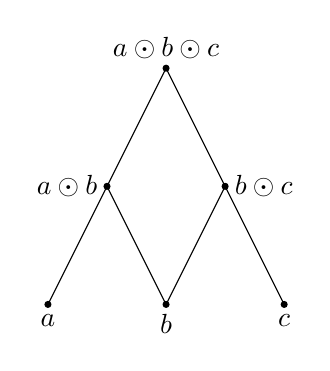
\begin{tikzpicture}[scale=.75]
	\draw[fill] (0,2) circle (.05cm) node[above]{$a \odot b \odot c$};
	\draw[fill] (-2,-2) circle (.05cm) node[below]{$a$};
	\draw[fill] (-1,0) circle (.05cm) node[left]{$a \odot b$};
	\draw[fill] (1,0) circle (.05cm) node[right]{$b \odot c$};
	\draw[fill] (2,-2) circle (.05cm) node[below]{$c$};
	\draw[fill] (0,-2) circle (.05cm) node[below]{$b$};

	\draw (-2,-2) -- (-1,0);
	\draw (0,-2) -- (-1,0);
	\draw (0,-2) -- (1,0);
	\draw (2,-2) -- (1,0);
	\draw (-1,0) -- (0,2);
	\draw (1,0) -- (0,2);
\end{tikzpicture}
\end{center}

\begin{center}
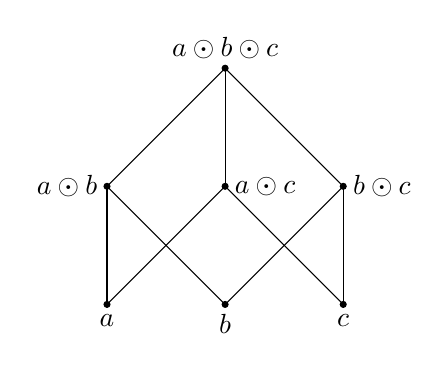
\begin{tikzpicture}[scale=.75]
	\draw[fill] (0,2) circle (.05cm) node[above]{$a \odot b \odot c$};
	\draw[fill] (-2,-2) circle (.05cm) node[below]{$a$};
	\draw[fill] (-2,0) circle (.05cm) node[left]{$a \odot b$};
	\draw[fill] (2,0) circle (.05cm) node[right]{$b \odot c$};
	\draw[fill] (2,-2) circle (.05cm) node[below]{$c$};
	\draw[fill] (0,-2) circle (.05cm) node[below]{$b$};
	\draw[fill] (0,0) circle (.05cm) node[right]{$a \odot c$};

	\draw (-2,-2) -- (-2,0);
	\draw (0,-2) -- (-2,0);
	\draw (0,-2) -- (2,0);
	\draw (2,-2) -- (2,0);
	\draw (-2,0) -- (0,2);
	\draw (2,0) -- (0,2);
	\draw (0,0) -- (-2,-2);
	\draw (0,0) -- (2,-2);
	\draw (0,0) -- (0,2);
\end{tikzpicture}
\end{center}

\end{document}
